% Chapter 3

\chapter{Cost Analysis, Conclusion, and Future Recommendations} % Write in your own chapter title
\label{Chapter5}
\lhead{} % Write in your own chapter title to set the page header

\section{Application in Communication Systems}
One of the major drawbacks of using the Neural Networks is that when the applications require a large amount of training data, the power and the specifications of the hardware required to go up exponentially. The more complexity we add to our model of the communication system, the more complicated becomes the architecture required. For example, in multi-user detection, when we moved from 16 subcarrier system to a more standard 64 sub-carrier systems, we had to increase the number of neurons by a factor of 4, and we had to increase the amount of training data by a factor of 10. The training required High-Performance Computing, and despite that, it took at least a week.  One positive outcome of this is that out of 2128 ($\approx 1038$) possible training messages which could be fed to our 64 subcarrier system, we at most require a very small subset of about tens of million distinct messages. This means that our network indeed learns the inverse of the transformation which mapped the bits to the received signal. Also, in terms of cost, big companies that are working in the field of communication do have powerful hardware at their disposal, which means that they will be able to train the network without the cost of any new hardware installation or purchase. One area of concern may be the power consumption of the hardware while training the network. But we must remember that we have to train the network only once to obtain the optimal weights of the model, which we can copy to and store in millions of devices. In other words, once we have trained the network, we can use a microcontroller or a chipset of negligible cost and power to do inference.


Nonetheless, it would be pertinent to mention that the system model our network uses is very rudimentary and simple. The neural network is trained at a constant SNR; the noise is AWGN, and the channel is drawn from a single Gaussian distribution; the bits are generated randomly too, and so the resultant symbols in the frame don’t have any covariance between them (On second thought, things could have been less complicated as covariance between symbols would have allowed us to use LSTM network who have a superior performance for sequence-2-sequence transformation.) To train our neural network for practical use, we could use more realistic channel models such as WINNER II. Also, we could change the SNR gradually but continuously to mimic real-time use of communication systems. Moreover, instead of generating the bits randomly, we could use data bits obtained from video, audio, or other documents to make the network more accurate. 

One area that has the potential for investigation is to decrease in pilot length. For Single-User Detection, when the pilot length is small, the performance of the neural network degrades less than that of traditional methods \cite{ye2018power}. Unfortunately, we failed to observe this trend for multi-user detection. Our future work aims to find improvements in the architecture, and find the optimal amount of training data so that we obtain this trend in the multi-user detection as well. 

\section{Application in Bioinformatics}
Our systems may have performed exceptionally well in terms of Area Under Receiver Operating Curve (AUC) as illustrated in Figure \ref{fig:third_res}, however, if we look at the sensitivity and specificity measures of the data as defined below:
$$Sensitivity = \frac{TP}{TP + FN}$$
$$Specificity = \frac{TN}{TN + FP}$$
In our context:
\begin{itemize}
\item $TP$ = True Positives = Number of Parkinson's Patients predicted as Parkinson's Patients
\item $TN$ = True Negatives = Number of Healthy People predicted as Healthy People
\item $FP$ = False Positives = Number of Parkinson's Patients predicted as Healthy People
\item $FN$ = False Negatives = Number of Healthy People predicted as Parkinson's Patients
\end{itemize}
Using this measure, we obtain the results illustrated in Figure \ref{fig:sens}. We see that they are not performing very well as the maximum sensitivity we were able to obtain is 0.41 which is not a very good result for providing a very good measure for providing Parkinson's predictions.
\begin{figure}[htbp]
  \centering
  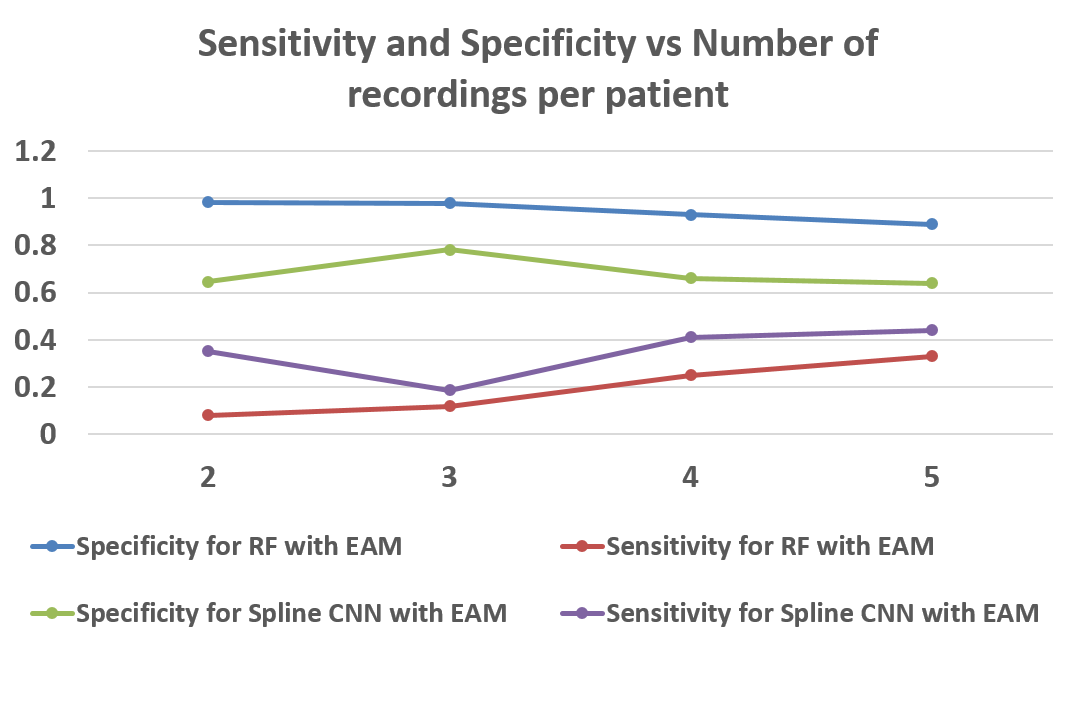
\includegraphics[width=\textwidth]{./Figures/park_sens_spec.png}
  \caption{Change in Sensitivity and Specificity as we change the number of recordings per person}
  \label{fig:sens}
\end{figure}
We believe that this is due to the following reasons:
\begin{itemize}
\item The data is highly imbalanced and stays so even when we change the recordings per patient as illustrated in Figure \ref{fig:fifth_res}. 
\item When we increase the number of recordings per patient, it seems to become less imbalanced, but at the same time, we have a lesser amount of data available, as there are fewer people who have recorded that many number of recordings or more. We can observe this trend in the number of recordings histogram in Figure \ref{fig:park_asymm}.
\end{itemize}
We aim to fight this trend either by optimizing our models for more sensitivity or by adding other modes (types) of activities data in the architecture as well. This way, the other activities data can help augment our predictions and improve them giving us a more robust model in terms of sensitivity and specificity as well.